%(brief description of the tasks and work packages that must be developed to achieve the goal of the project or study; identification of the dependencies amongst tasks; estimation of the necessary time to allocate to the tasks and preliminary TFG calendar (Gantt Chart or equivalent).

\section{Calendar}
\subsection{Description of the tasks}
A brief description of the tasks of this study can be found in the table \ref{taskssummary}.
\begin{longtable}{ | p{1.3cm} | p{3cm} | p{11cm} |}
\hline
\textbf{ID} & \textbf{Work Package} & \textbf{Brief task description list} \\ 
\hline
1 & State of the art & Research of the current computational methods used in the resolution of the conservation equations.\\ \hline
2 & \multicolumn{2}{|l|}{Conduction} \\ \hline
2.1 & Research on conduction & Research of the concept of conduction. \\ \hline
2.2 & Conduction code development & Development of a code in order to solve a conduction problem. \\ \hline
2.3 & Validation and analysis &  Validation of the conduction code and analysis of the results. \\ \hline
3 & \multicolumn{2}{|l|}{Convection} \\ \hline
3.1 & Research on convection & Research of the concept of convection. \\ \hline
3.2 & Convection code development & Development of a code in order to solve a convection problem. \\ \hline
3.3 & Validation and analysis &  Validation of the convection code and analysis of the results. \\ \hline
4 & \multicolumn{2}{|l|}{Radiation} \\ \hline
4.1 & Research on radiation & Research of the concept of radiation. \\ \hline
4.2 & Radiation code development & Development of a code in order to solve a radiation problem. \\ \hline
4.3 & Validation and analysis &  Validation of the radiation code and analysis of the results. \\ \hline
5 & \multicolumn{2}{|l|}{Combination: Conduction+Convection+Radiation} \\ \hline
5.1 & Combination code development & Development of a code that combines heat transfer by conduction, convection and radiation. \\ \hline
5.2 & Validation and analysis &  Validation of the code and analysis of the results. \\ \hline
6 & \multicolumn{2}{|l|}{Practical application} \\ \hline
6.1 & Research on the practical application & Selection and research of an engineering system that is going to be studied in order to understand the processes that are going to be simulated. \\ \hline
6.2 & Application code development & Development of a code to solve the particular application problem. \\ \hline
6.3 & Validation and analysis &  Validation of the code obtained and analysis of its results. \\ \hline
6.4 & Optimization &  Possible optimization of the engineering system studied. \\ \hline
7 & Conclusions & Writing of the final conclusions of the study. \\ \hline
\caption{Tasks Description}
\label{taskssummary}
\end{longtable}

\subsection{Dependencies among tasks}
\begin{longtable}{ | p{1.3cm} | p{7cm} | p{3cm} | p{3.5cm} |}
\hline

\textbf{ID }& \textbf{Task} & \textbf{Time (h)} & \textbf{Prelations} \\ \hline
0 & Beginning of the project & - & -  \\ \hline
1 & State of the art & 25 & 0 \\ \hline
2 & \multicolumn{3}{|l|}{Conduction} \\ \hline
2.1 & Research on conduction & 10 & 1 \\ \hline
2.2 & Conduction code development & 10 & 2.1 \\ \hline
2.3 & Validation and analysis & 5 & 2.2 \\ \hline
3 & \multicolumn{3}{|l|}{Convection} \\ \hline
3.1 & Research on convection & 25 & 1 \\ \hline
3.2 & Convection code development & 25 & 3.1 \\ \hline
3.3 & Validation and analysis & 10 & 3.2 \\ \hline
4 & \multicolumn{3}{|l|}{Radiation} \\ \hline
4.1 & Research on radiation & 15 & 1 \\ \hline
4.2 & Radiation code development & 15 & 4.1 \\ \hline
4.3 & Validation and analysis & 10 & 4.2 \\ \hline
5 & \multicolumn{3}{|l|}{Combination: Conduction+Convection+Radiation} \\ \hline
5.1 & Combination code development & 35 & 2; 3; 4 \\ \hline
5.2 & Validation and analysis & 10 & 5.1 \\ \hline
6 & \multicolumn{3}{|l|}{Practical application} \\ \hline
6.1 & Research on the practical application & 20 & 5 \\ \hline
6.2 & Application code development & 40 & 6.1  \\ \hline
6.3 & Validation and analysis & 15 & 6.2 \\ \hline
6.4 & Optimization  & 20 & 6.3 \\ \hline
7 & Conclusions & 10 & 6 \\ \hline
\caption{Prelations and time estimation} \\
\end{longtable}
To ensure a better comprehension of conduction, convection and radiation, they are not going to be studied at the same time but one after the other. 

\subsection{Gantt Chart}
\begin{figure}[h!]
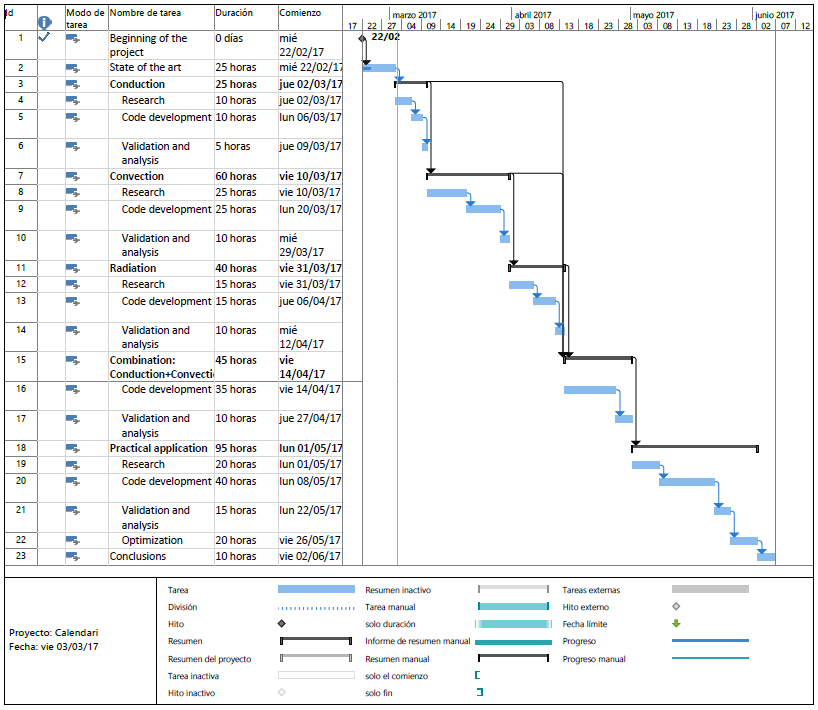
\includegraphics[scale=0.7]{Gantt}
\caption{Gantt Chart}
\end{figure}